\documentclass[11pt,a4paper]{article}
\usepackage[margin=2.5cm]{geometry}
\usepackage{booktabs}
\usepackage{listings}
\usepackage{xcolor}
\usepackage{graphicx}
\usepackage{float}

\lstset{
  basicstyle=\ttfamily\small,
  frame=single,
  backgroundcolor=\color{gray!8},
  breaklines=true
}

\title{Labwork 8: Scatter}
\author{Yanis Denizot -- 2640051}
\date{\today}

\begin{document}
\maketitle

\section{Implementation}
The input image is stored as an array of structures (AoS): each pixel keeps its R, G, B values
together, in an array of shape $(h, w, 3)$. The goal is to convert it to HSV and to store the
result as a structure of arrays (SoA): three separate 2D arrays \texttt{H}, \texttt{S} and
\texttt{V}. Then the second kernel does the opposite, from HSV (SoA) back to RGB (AoS).
Both kernels are 2D, with one thread per pixel ($16 \times 16$ blocks). I used Google Colab
(Tesla T4) and a $1200 \times 800$ image.

\textbf{RGB2HSV (scatter).} Each thread reads one pixel and writes its 3 values in 3 different
arrays. I used the formulas of the course: R, G, B are scaled to $[0, 1]$, then
$\Delta = max - min$, $V = max$, $S = \Delta / max$ (0 if $max = 0$), and $H$ depends on which
channel is the max. If $H$ is negative (red case), I add $360^\circ$, which is the same as the
``mod 6'' in the formula.
\begin{lstlisting}[language=Python]
if delta == 0:
    hue = 0.0
elif mx == r:
    hue = 60 * ((g - b) / delta)
elif mx == g:
    hue = 60 * ((b - r) / delta + 2)
else:
    hue = 60 * ((r - g) / delta + 4)
if hue < 0:
    hue = hue + 360
...
H[y, x] = hue
S[y, x] = sat
V[y, x] = mx
\end{lstlisting}

\textbf{HSV2RGB.} Each thread reads $H$, $S$, $V$ from the 3 arrays and writes one RGB pixel.
With $d = H / 60$, $h_i = \lfloor d \rfloor \bmod 6$ and $f = d - \lfloor d \rfloor$, I compute
$l$, $m$, $n$ like in the course, and choose $(R, G, B)$ from the 6 cases depending on $h_i$.
At the end the values are scaled back to $[0, 255]$. I add 0.5 before converting to
\texttt{uint8} to round to the nearest integer, otherwise a value like 254.9 becomes 254.
\begin{lstlisting}[language=Python]
dst[y, x, 0] = np.uint8(r * 255 + 0.5)
\end{lstlisting}

\section{Results}
After RGB $\rightarrow$ HSV $\rightarrow$ RGB, the output is exactly the same as the input
image (maximum difference = 0). The values are in the expected ranges: $H$ from 0 to
$359.7^\circ$, $S$ and $V$ from 0 to 1.

\begin{figure}[H]
\centering
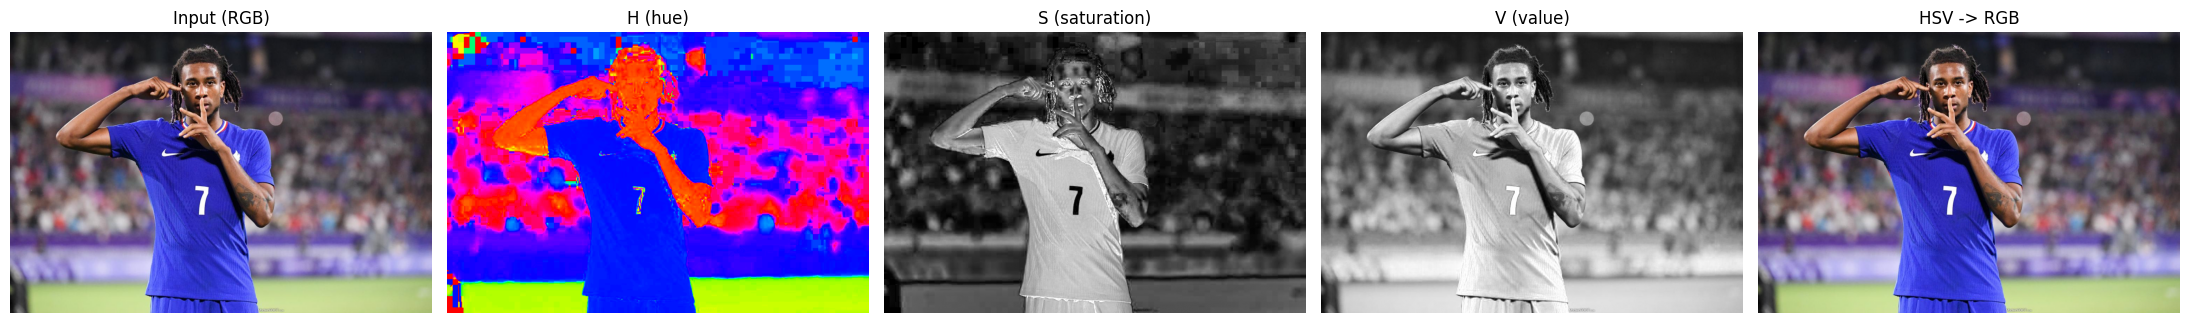
\includegraphics[width=\textwidth]{results.png}
\end{figure}

In the $H$ image, the jersey is blue and the grass is yellow-green. In the $S$ image the jersey
is white because its color is very saturated, and $V$ looks like a grayscale version of the
photo. The small squares in the background of $H$ come from the JPEG compression ($8 \times 8$
blocks): in dark and gray areas, small changes of R, G, B give big changes of hue.

\end{document}
